%%%%%%%%%%%%%%%%%%%%%%%%%%%%%%%%%%%%%%%%%%%%%%%%%%%%%%%%%%%%%%%%%%%%%%
%
% Autor: Jan Tulak
%
%%%%%%%%%%%%%%%%%%%%%%%%%%%%%%%%%%%%%%%%%%%%%%%%%%%%%%%%%%%%%%%%%%%%%%

\documentclass[12pt,a4paper,leqno]{article}
\usepackage[utf8]{inputenc}
\usepackage[czech]{babel}
\usepackage[T1]{fontenc}
\usepackage{times}
\usepackage[left=2cm,top=3cm,width=17cm,height=24cm,dvips]{geometry}
\providecommand{\uv}[1]{\quotedblbase #1\textquotedblleft}
\usepackage{verbatim}
\usepackage{amsmath}
\usepackage{amsthm}
\usepackage{amsfonts}
\usepackage{amssymb}
\usepackage{mdwlist}
\usepackage{graphics}
\usepackage{float}
\usepackage{multirow}
\usepackage{lscape}
\usepackage[breaklinks]{hyperref}
\usepackage{breakurl}
\usepackage{enumitem}
\usepackage{listings}
\usepackage{color}
\newcommand\red[1]{{\color{red}#1}}
\usepackage{mathtools}
\usepackage{picture}
\usepackage{float}
\usepackage{indentfirst}
\usepackage{epstopdf}

% roman numbers
\makeatletter
\newcommand*{\rom}[1]{\expandafter\@slowromancap\romannumeral #1@}
\makeatother


\let\chapter\undefined
\usepackage{tocloft}
\renewcommand{\cftsecleader}{\cftdotfill{\cftdotsep}}
%\renewcommand\cftsecfont{\normalfont}
%\renewcommand\cftsecpagefont{\normalfont}
%\renewcommand{\cftsecleader}{\cftdotfill{\cftsecdotsep}}
%\renewcommand\cftsecdotsep{\cftdot}
%\renewcommand\cftsubsecdotsep{\cftdot}
\newcommand{\eps}{\varepsilon}

\let\origappendix\appendix % save the existing appendix command
\renewcommand\appendix{\clearpage\pagenumbering{Roman}\origappendix}

\begin{document}
\thispagestyle{empty}
	\begin{center}
	\textsc{\LARGE Vysoké učení technické v Brně}\\[1,5mm]
	\textsc{\Large Fakulta informačních technologií}\\
	\vspace{\stretch{0.05}}
	\begin{figure}[!ht]
		\centering
		\scalebox{0.35}{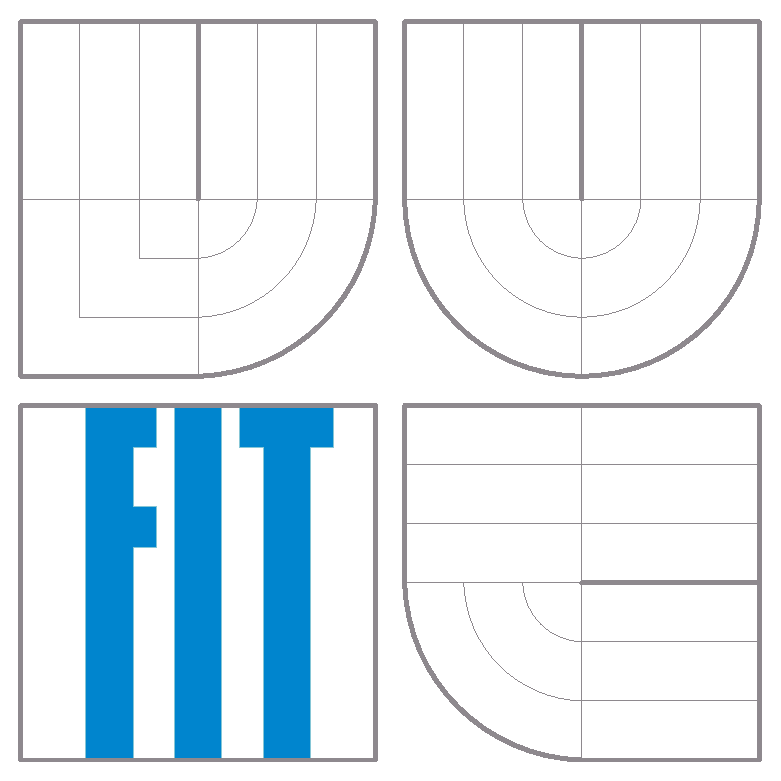
\includegraphics{logo}}
	\end{figure}
	\vspace{\stretch{0.05}}
	\LARGE{Teorie her a opensource}\\
	\vspace{\stretch{0.05}}
    \large{Zpráva do předmětu THE}
	\vspace{\stretch{0.618}}
	\end{center}
	{\Large{\textbf{Autor:}} Jan Ťulák (xtulak00)\vspace{5mm}}\\
	{\hfill \Large \today}\vspace{5mm}
\newpage
%%%%%%%%%%%%%%%%%%%%%%%%%%%%%%%%%%%%%%%%%%%%%%%%%%%%%%%%%%%%%%%%%%%%%%
%
% Author: Jan Tulak, xtulak00
%
%%%%%%%%%%%%%%%%%%%%%%%%%%%%%%%%%%%%%%%%%%%%%%%%%%%%%%%%%%%%%%%%%%%%%%

%%%%%%%%%%%%%%%%%%%%%%%%%%%%%%%%%%%%%%%%%%%%%%%%%%%%%%%%%%%%%%%%%%%%%%
\begin{abstract}
\noindent Navzdory stále rostoucímu významu open-source \todo{sources: microsoft opening, apple based on, millenials and jobs...} v ekonomice je obtížné nalézt články či výzkumy zaobírající se studiem open-source z pohledu teorie her. A to jak z pohledu ekonomického (soupeření open-source a proprietárních produktů či dodavatelů), tak z pohledu spíše psychologického (pohled na jednotlivé členy open-source komunity, jejich motivaci, očekávaný zisk, a podobně.) Nějaký výzkum v této oblasti však přeci jen existuje a v této zprávě se tedy pokouším shrnout některé dostupné materiály k tématu.
\end{abstract}

\listoftodos
\hrulefill
\begin{multicols}{2}
\lettrine[nindent=0em,lines=3]{O}{pen source} ve smyslu definovaném Open Source Initiative~\cite{OSI-2011}, znamená svobodný přístup, distribuci a modifikaci.\todo{Some opening, more about used sources...} V takovém prostředí je velmi obtížné, až nemožné, pro nějakou skupinu či jednotlivce získat dominantní postavení. Konkrétní vývojář sice může uplatňovat sebetvrdší pravidla a vést svůj projekt určitým způsobem, nemůže však nikomu zabránit ve vytvoření paralelního projektu sdílejícího stejný kód (tzv. vytvořit fork) a vést vývoj jiným směrem. A bude-li tento nový směr přijatelnější pro uživatele či přispěvatele do projektu, původní projekt může zaniknout, aniž by přitom do něj vložená práce byla ztracena.

Open source se přitom zásadně liší od zažitých představ a předpokladů a softwarovém vývoji a nabourává dosavadní teorie o motivaci inovovat~\cite{promise-of-research-opensource}. Toto se dá snadno ilustrovat na Vězňově dilematu. Klasická verze hry, kdy hráči rozhodují, jestli zveřejnit svůj vývoj, nebo ho držet uzavřený, se dá popsat podle hry v tabulce \ref{tab:classic-prisoner}. V takové hře je sice spolupráce na otevřeném projektu pro oba hráče lepší, než když každý z nich pracuje na své uzavřené variantě. Ale protože většího zisku hráč dosáhne, pokud použije data zveřejněná konkurentem a sám nic nepřispěje (a konkurent tak kvůli delšímu vývoji získá méně zákazníků), má takováto hra jediné Nashovo ekvilibrium (uzavřít,uzavřít), tedy zisk $(-1,-1)$.

\begin{Figure}
\begin{center}
\begin{tabular}{r| c c}
		& Otevřít & Uzavřít \\
		\hline
	Otevřít & $1,1$ & $-2,2$ \\
	Uzavřít & $2,-2$ &\cellcolor{gray!20}  $-1,-1$ \\
\end{tabular}
\end{center}
\captionof{table}{Klasická představa hry o otevřenost vývoje.}
\label{tab:classic-prisoner}
\end{Figure}

Pokud ale budeme uvažovat modifikovanou variantu, situace se změní. Řekněme, že zisk pro hráče je jeho původní zisk plus polovina zisku soupeře.

\begin{Figure}
\begin{center}
\begin{tabular}{r| c c}
		& Otevřít & Uzavřít \\
		\hline
	Otevřít &\cellcolor{gray!20}  $1.5,1.5$ & $-1,1$ \\
	Uzavřít & $1,-1$ &\cellcolor{gray!20}  $-1.5,-1.5$ \\
\end{tabular}
\end{center}
\captionof{table}{Upravená verze hry o otevřenost vývoje.}
\label{tab:new-prisoner}
\end{Figure}

Tato verze hry, podle tabulky~\ref{tab:new-prisoner}, má Nashova ekvilibria dvě. Stále zůstává (uzavřít,uzavřít), nicméně (otevřít,otevřít) je nyní také ekvilibrium, které navíc poskytuje vůbec největší zisk pro každého hráče~\cite{network-effects-opensource}.

Jaký model lépe vystihuje skutečnost není jasné. Zřejmě však silně záleží na konkrétním trhu, situaci, a jak je vidět v kapitole~\ref{ch:opensource-vs-proprietary}, chování zákazníků. V kapitole~\ref{ch:architecture-opensource} si ukážeme ještě jiný alternativní model, který neuvažuje soupeření, a tedy zisk hráče je stejný (odpovídá námaze na vytvoření), ať už jeho protihráč jeho kód využije, či ne.

Protože tato zpráva vznikla jako shrnutí několika různých textů, které se věnují různým aspektům problematiky, rozdělil jsem ji do kapitol odpovídajících daným zdrojům. Každá kapitola je tedy shrnutím jednoho či více zdrojů, s dodatečnými informacemi a zdroji.




%%%%%%%%%%%%%%%%%%%%%%%%%%%%%%%%%%%%%%%%%%%%%%%%%%%%%%%%%%%%%%%%%%%%%%
\section{Open-source vs proprietární software}
\label{ch:opensource-vs-proprietary}
	{\em Tato kapitola vychází ze zprávy Lock-In Strategy in Software Competition, K. Zhu a Z. Zhou~\cite{lock-in-competition}.}

	Podle dotazníku provedeného Computer World v roce 2004 byl \uv{vendor lock-in}\footnote{{\em Vendor lock-in} popisuje situaci, kdy zákazník je nucen pokračovat v užívání konkrétního produktu/dodavatele i při existenci alternativ, protože přechod na jiné řešení či jiného dodavatele by byl pro zákazníka velmi nákladný. Možností, jak může dodavatel lock-in dosáhnout je vícero: (1) systém je navržen tak, aby nebyl kompatibilní s alternativními řešeními od ostatních dodavatelů; (2) využíváním uzavřených architektur a proprietárních standardů; (3) Licenční a patentovou politikou.} jednou z hlavních obav mezi IT odborníky ohledně nastupujícího trendu cloud computingu~\cite{computer-world-2004}. Ve výzkumu provedeném North Bridge v roce 2015 je snaha vyhnout se vendor lock-in zmiňována jako jeden z důvodů pro výběr open-source řešení~\cite{survey-2015}.

	Zatím co pro dodavatele je \uv{lock-in} obvykle přínosný, neboť snižuje
	vyjednávací sílu zákazníka a může umožnit až monopolní postavení i na trhu,
	kde existuje konkurence~\cite[str. 1]{lock-in-competition}, pro zákazníka
	je tomu ze zřejmých důvodů naopak. Intuitivně se zdá, že dodavatelé
	uzavřeného software by měli vždy preferovat lock-in. Paul Klemperer však ve
	svém článku (1986) ukazuje na duopolistickém soupeření se dvěmi obdobími
	(\uv{aktuální období} a \uv{budoucí období}) a cenou za změnu dodavatele, že v soupeření o zákazníka mohou dodavatelé nabízet takové slevy pro první období, že celkový zisk z druhého, udržovacího období už nevyrovná ztrátu z prvního~\cite{klemperer-switching-costs,lock-in-competition}.

	Současně obavy z lock-in posilují pozici open-source hnutí v softwarovém průmyslu, protože zákazníci jej vidí jako možnost, jak snížit svou závislost na jednom proprietárním dodavateli~\cite{opensource-advantage}. Podle průzkumu provedeného Computer Economics (2005) je hlavní výhodou použití open source nikoliv snížení nákladů, ale právě snížení závislosti. Podstatným důvodem je, open source neumožňuje vynucený upgrade a software může být podporován a opravován otevřenou komunitou. Konkurence v komunitě snižuje cenu za podporu a udržování staršího software. Naproti tomu výrobci proprietárního software mohou často vydávat nové verze software a ukončovat podporu starších verzí. Tím nutí zákazníky k (často placenému) upgrade a zákazník je na takovém výrobci závislý, neboť jeho jediná alternativa je zůstat s nepodporovanou verzí. Open Source Initiative tvrdí, že \uv{the promise of open source is ... an end to predatory vendor lock-in.}~\cite{OSI} ({\em Příslib open source je ... konec predátorského lock-in.})

	Autoři studie popisované v této kapitole vytvořili dvou-obdobní model inspirovaný prací P. Klempera. V tomto modelu se zákazníci odlišují mezi sebou svými preferencemi a model zahrnuje open source a {\em nestrategický\footnote{Cenu proprietárního software strategicky stanovuje jeho dodavatel. Otevřená komunita se nechová strategicky, nebude tedy lákat zákazníky na nízkou cenu v prvním období, kterou by následně zvýšila~\cite[str. 2]{lock-in-competition}.}, ale důvěryhodný závazek} o budoucích cenách (tj. cena vždy zůstane zdarma), garantovaný OSS licencemi, jako je třeba GNU General Public License (GPL)\footnote{Zde považuji za nutné zdůraznit, že GNU GPL nezakazuje prodej SW~\cite{selling-foss}. Protože však autor nemůže s takovouto zabránit volnému šíření, může se např. několik potenciálních zákazníků spojit a software zakoupit společně. V praxi tedy nemůže nastat situace s monopolní cenou produktu. Pokud ale ani autor, ani žádný zákazník neposkytne získaný software zdarma někomu dalšímu, cena nemůže být nulová.}~\cite[str. 2]{lock-in-competition}. Rovněž protože zákazník má k dispozici zdrojové kódy a může je dále šířit a modifikovat, nemůže nikdo získat monopolní postavení pro upgrade a podporu.

	Tento závazek open source způsobuje problém pro dodavatele uzavřených řešení, neboť je obtížnější zajmout zákazníka přemýšlejícího o budoucnosti, který může vycícit riziko lock-in. Pokud tedy má vybrat proprietární produkt s očekáváním lock-in, bude takový zákazník chtít výraznou slevu, či dokonce dotaci před pořízením takového produktu. Takové slevy pro získání zákazníků mohou nakonec dodavatele stát víc, než kolik následně na lock-in vydělá v druhé fázi, jak autoři ukazují na svém modelu. Konkrétní ztráta či zisk se však liší, pokud zákazník plánuje jen krátkou dobu dopředu. V takovém případě může být lock-in pro dodavatele výhodný.

	Následující podkapitola popisuje použitý model a jeho předpoklady.

	\subsection*{Model}
	{\em Tato podkapitola je zkráceným překladem. Zdroje jsou uvedeny tak jako v původním textu.}

	Dva dodavatelé software soupeří na jednom trhu. Licencují svůj software pro dvě období, konkrétně současnost a budoucnost. Ceny oznamují současně na začátku každého období. Dodavatelé nemohou nastavit odlišné ceny různým typům zákazníků, protože typ je zákazníkova privátní informace, dodavatelé jej neznají. Software je označen A, nebo O, kde A znamená proprietární software a O je open source. Je známo, že softwarové produkty mají nízké nebo nulové mezní náklady\footnote{Náklady při výrobě dodatečné jednotky produktu, v tomto případě prodeji jedné licence.} (Shapiro a Varian 1999). Pro technické zjednodušení, mezní náklady obou dodavatelů byly normalizovány na nulu. Protože open source může být získán zdarma či za velmi nízkou cenu (zaslání DVD, ...), předpokládáme, že:

	\vspace{10pt}
	\noindent{\sc Předpoklad 1.}~{\em Cena získání OSS je normalizována na nulu.}
	\vspace{10pt}

	Nechť $p_{it}: i \in {A,O}, t \in {1,2}$ značí cenu získání software $i$ v období $t$. Z předpokladu 1 máme $p_{O1} = p_{O2} = 0$. Protože $p_{O1}$ a $p_{O2}$ nejsou v této zprávě strategické rozhodovací proměnné, nastavujeme je na nulu. Později ukážeme, že i pokud bychom nastavili jejich hodnotu na pozitivní nenulovou konstantu, neovlivní to podstatně výsledek.

	Open source a proprietární software jsou jasně rozlišené. Schmidt a Schnitzer (2002) toto rozlišení modelovali jako horizontální odlišnost\footnote{{\em Horizontal differentiation} -- situace, kdy odlišnost dvou produktů nelze jednoduše ohodnotit např. kvalitativně. Příkladem může být třeba kvalitativně totožný produkt nabízený ve dvou barevných provedeních. Lze rovněž definovat jako {\em\uv{pokud jsou všechny varianty nabízeny za stejnou cenu, je nenulová poptávka po každé z nich}} (Cremer a Thisse 1991, p. 383). Vertikální odlišnost pak poskytuje jednoznačně ohodnotitelné a uspořádatelné srovnání.}. Podle literatury (Caminal a Matutes 1990, Klemperer 1995, Marinoso 2001) zahrnujeme tento rozdíl pomocí {\em modelu horizontální odlišnosti}.

	\vspace{10pt}
	\noindent{\sc Předpoklad 2.}~{\em OSS a proprietární software jsou horizontálně odlišné.}
	\vspace{10pt}

	Tedy pokud $A$ i $O$ jsou nabízeny za stejnou cenu, někteří zákazníci zvolí $A$, zatímco jiní $O$, protože jinak hodnotí vlastnosti produktu. Například OSS lze snadněji upravit pro konkrétní potřeby, zatímco proprietární software mívá kvalitnější uživatelské rozhraní a dokumentaci. Jako příklad může posloužit srovnání J2EE a .NET. Estes a Maxime (2003) shrnují seznam srovnání mezi J2EE a .NET a konstatují, že výběr záleží na konkrétních potřebách a preferencích  uživatele.

	Motivování takovým pozorovnáním v praxi, přidáváme další rozměr heterogenity: {\em reservation utility}\footnote{Pro {\em reservation utility} se mi nepodařilo nalézt vhodné české slovo. Význam tohoto pojmu by se dal volně větou přeložit jako \uv{využití nasmlouvané kapacity}. V případě SW to odpovídá intenzitě využívání a případně i počtu licencí.}\todo{Czech translation?}, což náš model činí dvourozměrným, na rozdíl od literatury, která používá jednorozměrný horizontální, příp. jednorozměrný vertikální model odlišnosti. Pro každý software totiž mají různí zákazníci různé využití. Někteří jej využívají intenzivně, pro jiné je jen okrajovým nástrojem. To vede k odlišné {\em reservation utility} mezi zákazníky kvůli jejich rozdílům v ohodnocení, rozpočtu, či ceně. (Gartner Researarch Note 2003).

	\vspace{10pt}
	\noindent{\sc Předpoklad 3.}~{\em Zákazníci mají vertikálně odlišnou svou reservation utitlity.}
	\vspace{10pt}

	Protože model zachycuje heterogenitu ve dvou dimenzích, jsou zákazníci matematicky modelování jako dvojice $r$ a $\theta$, kde $r$ představuje reservation utility a $\theta$, nezávisle na $r$, vzdálenost jejich preference od produktu $A$ (tedy $(1-\theta)$ je vzdálenost od $O$.) Zákazníci jsou uniformě distribuovaní v rozsahu $[0,1]$ pro $\theta$ a pro $r$ v rozsahu $[R, (1+\lambda)R]$, kde $1/\lambda R$ je funkce hustoty, kde $R$ je spodní hranice zákazníkovy reservation utility.

		\vspace{10pt}
		\noindent{\sc Předpoklad 4.}~{\em Zákazníci jsou reprezentováni $(r,\theta)$, kde $\theta \sim U(0,1)$ a $r \sim U(R, R(1+\lambda))$.}
		\vspace{10pt}

	Pokud zákazník $(r,\theta)$ vybere řešení $A$, pak jeho zisk je $r-\theta - p_{At})$ pro období $t$. Pokud si vybere $O$, pak jeho zisk je $r-(1-\theta)$. Pokud si nevybere nic, jeho zisk je nula. {\em Celkový zisk} je suma zisků za obě období.

	Ve hře jsou dvě období. Na začátku prvního oba dodavatelé zároveň oznámí svou cenu $p_{i1}$. Zákazníci si vytvoří racionální odhadad ceny $p_{i2}$ pro další období, porovnají celkové zisky za obě periody a vyberou si jedno řešení. Ve druhém období dodavatelé provedou upgrade svého software a zaúčtují zákazníkům $p_{i2}$. Zákazník může nadále platit za dříve vybrané řešení, zrušit předplatné (a využívat starou verzi), nebo přejít k druhému řešení.

		\vspace{10pt}
		\noindent{\sc Předpoklad 5.}~{\em Zákazník při přechodu na jiný než původně vybraný software bude muset zaplatit cenu $s (s\geq0)$.}
		\vspace{10pt}

	Tato cena za přechod představuje náklady na změnu nastavení hardware, přepsaní vlastních úprav a aplikací, přeškolení zaměstnanců. Dodavatelé v druhém období upgradují svůj SW, což zvýší zákazníkovu reservation utility o $v_{up}\geq0$. Pokud zákazník zůstane u zvoleného řešení, jeho zisk je $0\leq v_b < R$. Předpokládáme, že zákazník využívá v daném období pouze jeden produkt.

	\subsection*{Výsledky modelu}
	{\em V této kapitole shrnuji výsledky získané z výše popsaného modelu, což zahrnuje kapitoly 3, 4, 5 a 6 původní zprávy.}

	Nejprve se zaměřme na do budoucna uvažující zákazníky, kteří očekávají, že v případě $A$ budou platit v druhém období vyšší cenu. Pokud dodavatel $A$ dokáže správně nastavit své ceny, pak ve druhém období žádný zákazník nezmění využívaný produkt z $A$ na $O$, ale ani opačně, neboť zákazníci, kteří si $A$ vybrali, takové zvýšení předpokládali a započítali ho k ceně v prvním období. V případě zákazníků, kteří si naopak vybrali $O$ žádný důvod k přechodu není, neboť jejich cena se nezměnila~\cite[kap. 3: Lemma 1]{lock-in-competition}.

	Autoři ukazují, že zákazníci, kteří nejpravděpodobněji přejdou od $A$ k $O$ při neoptimální ceně jsou převážně zákazníci s vysokou reservation utility, tedy zákazníci pro dodavatele důležití.

	Přesto, že při optimálních cenách nedojde ke změně, někteří zákazníci, s nízkou reservation utility, mohou odmítnout upgrade a zůstat na staré verzi, tedy nepřinést v období 2 žádný zisk. To se týká především těch zákazníků, kteří jsou indiferentní mezi $A$ a $O$, a přesto, že ví, že si variantu $A$ z nějakého důvodu nemůžou v období 2 dovolit, sleva v období 1 je přiměje vybrat si produkt $A$~\cite[str. 6]{lock-in-competition}.

	Důsledkem je, že celkový zisk dodavatele $A$ je ve hře, kde ne všichni jeho zákazníci upgradují nižší, než by byl ve hře bez, nebo s nízkou cenou za přechod. Důvodem je, že sice vyšší cena za přechod dovolí dodavateli $A$ účtovat v období 2 vyšší cenu, ale aby získal zákazníky, musí v prvním období nabídnout slevu. Jenže nízká cena v období 1 nenaláká pouze užitečné zákazníky s vysokým reservation utility, ale také \uv{neužitečné}, kteří využijí nízké ceny na úkor dodavatele, ale už nepřinesou žádný následný zisk.

	Pokud ale cena za přechod je nízká či žádná, dodavatel nemůže v období 2 výrazně zvednou cenu. Zákazníci se tak nemusí obávat, že je dodavatel $A$ ve druhém období zneužije a ochotněji přijmou jeho řešení s vědomím, že kdykoliv mohou jít ke konkurenci. Důsledek je, že $A$ nemusí snižovat v prvním období svůj zisk, a tedy nabídnutí možnosti volby zákazníkům je pro něj paradoxně přínosnější~\cite[str. 7 a kap. 3: lemma 2]{lock-in-competition}.

	Model tedy ukazuje, že vendor lock-in v soupeření s Open Source řešením proprietárního dodavatele poškozuje.

	Pokud rozšíříme pohled i na krátkozraké zákazníky\footnote{Krátkozrakým zákazníkem může být například společnost, kde o výběru řešení rozhoduje pracovník, který předpokládá, že v druhém období už nebude v dané společnosti pracovat, a jehož plat či odměna závisí na zisku z prvního období.}, zjistíme, že ti ve svém rozhodování nijak neuvažují následující období a rozhodují se čistě podle cen v první periodě. V takovém případě je pro dodavatele $A$ jednoznačně výhodnější vendor lock-in použít. Je tedy vidět, že chování zákazníků má výrazný vliv na ekvilibrium hry~\cite[kap. 4]{lock-in-competition}.

	Celkový zisk všech zákazníků ve hře byl v případě, že dodavatel $A$ použil lock-in nižší, než pokud měli zákazníci možnost volby~\cite[kap. 5]{lock-in-competition}

	Výsledky tohoto modelu potvrzuje vývoj průmyslu ve zvyšování interoperability mezi proprietárním a Open Source software, jako příklad můžeme použít stále rostoucí příklon či spolupráci s Open Source u Microsoftu a Oracle~\cite[kap. 6]{lock-in-competition}, nebo úspěch Red Hatu~\cite{redhat-growth}.

%%%%%%%%%%%%%%%%%%%%%%%%%%%%%%%%%%%%%%%%%%%%%%%%%%%%%%%%%%%%%%%%%%%%%%
\section{Vliv architektury systému na vývojový proces v open-source}
\label{ch:architecture-opensource}
	{\em Tato kapitola vychází z článku The Architecture of Participation od C. Baldwin a K. Clark~\cite{architecture-opensource}.}

	Autoři tohoto článku si kladou otázku, jaký vliv má modularita (či monolitičnost) na atraktivitu daného projektu pro další vývojáře, kteří se potenciálně mohou zapojit do vývoje. Modularitu pro účely tohoto článku definují tak, že {\em komplexní systém vykazuje modularitu v návrhu, jestliže jeho části mohou být implementovány nezávisle, ale pracují společně a podporují celek.} Tato modularita nemusí být nutně reflektována {\em runtime} modularitou výsledného kódu~\cite[kap. 2.1]{architecture-opensource}

	Dále autoři pracují s rozdělením kódu na {\em platformu} a sadu modulů. Platforma poskytuje podporu modulům a je kritickou částí systému. Moduly jsou odlišné části většího systému, které mohou být implementovány nezávisle při dodržení jistých pravidel. Tato definice je použita pro určení odlišných částí systému, nespecifikuje žádnou konkrétní architekturu. V extrémním případě lze říct, že monolitický projekt má platformu a moduly integrované do jednoho nedělitelného celku.

	\subsection*{Nedobrovolný altruismus}
	Ve svém modelu autoři využívají pojem {\em nedobrovolný altruismus}. Ten lze charakterizovat tak, že práce každého hráče přispěje pozitivně k zisku všech ostatních bez ohledu na to, zda daný hráč chce ostatním pomoci, či ne~\cite[kap. 3]{architecture-opensource}. To reflektuje situaci, kdy jeden hráč vytvoří nějaký software, který je volně zveřejněn, a který může kdokoliv využít aniž by tím jakkoliv ovlivnil zisk autora. Nejlépe to lze ilustrovat hrou v tabulce~\ref{tab:involuntary-altruism-nf}. Hráč má zisk $v$ z použití nějakého software, a cena za vytvoření takového software je $c$. Předpokládáme, že $v > c$, takže pokud by byli hráči izolovaní, vytvořili by oba svou verzi daného programu.

	\begin{Figure}
	\begin{center}
	\begin{tabular}{r| c c}
			& Použít cizí & Vytvořit \\
			\hline
		Použít cizí & $0,0$ &\cellcolor{gray!20} $v, v-c$ \\
		Vytvořit &\cellcolor{gray!20} $v-c, v$ & $v-c, v-c$ \\
	\end{tabular}
	\end{center}
	\captionof{table}{Normální forma jednoduché hry nedobrovolného altruismu. Symetrická, jednokolová hra dvou hráčů.}
	\label{tab:involuntary-altruism-nf}
	\end{Figure}

	Tato hra má dvě Nashova ekvilibria v ryzích strategiích, kdy jeden vývojář pracuje, a druhý využije jeho kód. Tato ekvilibria jsou efektivní, tedy maximalizují zisk a minimalizují náklady, ale jsou nespravedlivá -- jeden vývojář se ,,veze'' na práci druhého. Je zde ale také smíšené ekvilibrium, kde  každý hráč pracuje s pravděpodobností $\alpha^* = 1-c/v$. S rostoucím počtem hráčů se situace nijak výrazně nemění. Veškerou práci stále provede jeden z nich a ostatní ji jen využijí.

	Problémem této hry je, že hráč, který program vytvoří, nemá z jeho zveřejnění žádný užitek, jeho zisk je stejný, jako kdyby hrál sám. Obrazem této hry ve skutečnosti pak je silně modulární program, kde jakákoliv změna výrazně ovlivní ostatní části systému. Taková situace vyžaduje hluboké znalosti celku, což odrazuje potenciální přispěvatele, a rovněž autor se bude zdráhat přijmout cizí úpravy.

	Na druhou stranu, u modulárních systémů může autor jednoho modulu profitovat z kódu napsaného jiným hráčem pro jiný modul. Je tedy na první pohled patrné, že modulární architektura vytváří příležitosti pro spolupráci vývojářů na různých částech systému.

	Uvažujme nyní hru dvou hráčů s perfektní informací. Systém, který chtějí hráči použít, zahrnuje platformu a dva moduly, $A$ a $B$. Platforma je v době hry již napsaná a tedy cena za její vytvoření již není podstatná. Moduly je však třeba vytvořit.


		\begin{Figure}
		\begin{center}
		\begingroup
		\medmuskip=0mu
		\thickmuskip=0mu
			\makeatletter\def\f@size{8}
		\hskip-0.7cm
		\begin{tabular}{r| c c c}
				& $Nic$ & $A$ & $B$ \\
				\hline
			$Nic$ &
			 	$0,0$ &
				$\frac{1}{2}v, \frac{1}{2}(v-c)$ &
				$\frac{1}{2}v, \frac{1}{2}(v-c)$ \\
			$A$ &
				$\frac{1}{2}(v-c), \frac{1}{2}v$ &
				$\frac{1}{2}(v-c), \frac{1}{2}(v-c)$ &
				\cellcolor{gray!20}$v-\frac{1}{2}c, v-\frac{1}{2}c$ \\
			$B$ &
				$\frac{1}{2}(v-c), \frac{1}{2}v$ &
				\cellcolor{gray!20}$v-\frac{1}{2}c, v-\frac{1}{2}c$ &
				$\frac{1}{2}(v-c), \frac{1}{2}(v-c)$ \\
		\end{tabular}
		\endgroup
		\end{center}
		\captionof{table}{Normální forma jednoduché hry nedobrovolného altruismu dvou hráčů se dvěma moduly.}
		\label{tab:involuntary-altruism-modules-perfect-information}
		\end{Figure}

	Z definice modulů je možné na každém z nich pracovat nezávisle. Každý z těchto modulů zvedne hodnotu systému o $v/2$ za cenu $c/2$. Celkem tak zisk celého systému zůstává $v$ a náklady $c$, jako u monolitického systému. Rozdíl však je, že platforma a libovolný modul je funkční celek, a lze mít zisk ze systému i pokud ne všechny moduly jsou implementovány.

	Každý hráč si může nezávisle vybrat, za nebude vytvářet nic, či zda vytvoří modul $A$, či $B$.

	Výsledná hra je zobrazena v tabulce~\ref{tab:involuntary-altruism-modules-perfect-information}. Hra má dvě Nashova ekvilibria (zvýrazněno šedou barvou), ve kterých si hráči rozdělí práci na modulech. V těchto ekvilibriích je pro oba vývojáře jednoznačně výhodnější se do vývoje zapojit, než zůstat stranou a buď se jen vézt, nebo implementovat nezávislé řešení. Jejich zisk je totiž $v - c/2$, oproti $v-c$ pro izolovanou činnost.

	Po zobecnění této hry na hru N hráčů a $j$ kol autoři dokazují dvě tvrzení: (1) Že ve hře s úplnou informací a ryzími strategiemi budou všechny moduly vytvořeny právě jednou. (2) A že nespravedlivá ekvilibria, kde není práce rovnoměrně rozdělena mezi hráče, nejsou sub-game perfektní.

	Důkaz prvního tvrzení je veden proti strategickému profilu, kde některý modul není naprogramován. Zřejmě v takovém profilu může některý hráč, který nic nedělá, zlepšit svůj zisk tím, že chybějící modul naprogramuje. Tedy takový profil nemůže být ekvilibriem.

	Druhé tvrzení pak dokazují na příkladu s různě ochotnými vývojáři, kdy někteří čekají, jestli za ně neudělá práci někdo jiný, zatímco další začnou pracovat ihned a v každém kole naprogramují jeden modul. Tato situace se dá chápat jako hrozba (,,nebudu pracovat''), ovšem je hrozbou nedůvěryhodnou, neboť v posledním kole tito hráči musí naprogramovat nějaký modul, jak bylo ukazuje předchozí tvrzení. V takové situaci je ovšem i pro vývojáře, kteří by začali pracovat hned, lepší počkat na poslední kolo stejně jako ostatní~\cite[kap. 4.1]{architecture-opensource}.

	V souhrnu pak taková hra s $N$ hráči a $j$ moduly a koly (tedy je možné, aby pro $N =1$ byl naprogramován celý systém se všemy moduly) má vždy co nejrovnoměrnější rozdělení práce. Počet hráčů, kteří se pouze vezou, však nemá na aktivní vývojáře žádný vliv. Pokud $N > j$, tedy je více hráčů než modulů, zisk vývojářů se nijak nezmění oproti $N = j$.

	\subsection*{Hodnota volby}
%%%%%%%%%%%%%%%%%%%%%%%%%%%%%%%%%%%%%%%%%%%%%%%%%%%%%%%%%%%%%%%%%%%%%%
\section{Shrnutí}







%%%%%%%%%%%%%%%%%%%%%%%%%%%%%%%%%%%%%%%%%%%%%%%%%%%%%%%%%%%%%%%%%%%%%%
%\section{Zdroje}
\bibliographystyle{czechiso}
%\bibliographystyle{plain}
%\begin{flushleft}
\bibliography{proj}
%\end{flushleft}
\end{multicols}
%\section{Přílohy}

\end{document}
